\documentclass[10pt,twocolumn]{article}
\usepackage{graphicx}
\usepackage{amsmath}
\usepackage{booktabs}
\usepackage[margin=0.5in, top=0.2in, bottom=0.5in]{geometry}
\usepackage{authblk}
\usepackage{hyperref}
\usepackage{float}
\usepackage{caption}
\usepackage{subcaption}
\usepackage{cleveref}

\usepackage{siunitx}

% Handle figures in two-column layout better
\usepackage{stfloats}

% Title formatting
\title{\Large \textbf{Neuron Responses to Grating Stimulus Orientations in Mice}}

\author{
  Umut Tuna Akgul, Utku Bahcivanoglu, Tommaso Ferracina, George Morris, Tebe Nigrelli
}


\begin{document}

\maketitle

\begin{abstract}
We analyze ecephys data from the Allen Brain Observatory to investigate how neural units in the mouse visual cortex respond to static and drifting gratings stimuli. We identify brain regions and specific neurons that have a significant role in encoding stimulus orientation. We combine neural firing rate over multiple trials and conditions, and select the most informative neurons based on their response. Finally, we construct an effective decoder to predict stimulus orientation from neural activity.
\end{abstract}


\section{Data Processing}

For our analysis, we chose \cite{Allen:750332458} for its balanced distribution of units across regions of the brain, and for its coverage of the visual cortex [Table \ref{tab:regions}].  This dataset consists of time-aligned responses of neuronal units to stimuli.

In this study we look at static and drifting grating presentations, and consider as the variable only the orientation and as the response only the mean firing rate of individual units over each presentation.

\section{Exploratory Data Analysis}

Due to the visible linear relation between the mean and the standard deviation of firing rates, it is intuitively true that they do not sufficiently characterize the brain regions [Figure \ref{fig:firing_rate_stats}].  Furthermore, as some regions contain little data, any possible spread is subject to noise [Figure \ref{fig:firing_rate_single}].

\textit{And then what?}

\subsection{Decoding static vs drifting}

A Wilcoxon signed-rank test indicated that for units in the \texttt{VISam} region of the visual cortex, the average spike rate over static presentations was higher than over drifting presentations (Figure \ref{fig:spike_mean}, \(z=0.0\), \(p<.001\)), and the coefficient of variation lower (\ref{fig:spike_cv}, \(z=16.0\), \(p<.001\)).

\section{Selection of Neurons}

For selecting units with high sensitivity to orientation differences, we define the Orientation Selectivity Index (OSI) of a unit,
\[\textrm{OSI} = \frac{r_{\theta^*} - r_{\bar\theta}}{r_{\theta^*} + r_{\bar\theta}}\]
where \(r_\alpha\) is the average firing rate of a unit over presentations with orientation \alpha, \(\theta^*\) is the value which maximizes \(r_{\theta^*}\), and \(\bar\theta\) is the angle orthogonal to \(\theta^*\).

We identify and select a highly selective subset of units with \(\textrm{OSI} > .5\).  Furthermore, we select units which have unequal firing rates throughout orientations with a one-way ANOVA test (\(\alpha = 0.05\)).  Finally, we narrow the list of units we look at to those which both have high OSI values and for those which have an unequal distribution.

\subsection{Static}

Our approach when looking at static stimuli yielded 43 units, which showed notable concentrations in the Visual Cortex, specifically the \texttt{VISal} and \texttt{VISl} areas [Table \ref{tab:chosen-regions-static}].  The anatomical distribution of these neurons aligns with established literature on the hierarchical organization of orientation processing in the mouse brain.

Visualization of orientation tuning curves from representative neurons [Figure \ref{fig:static_tuning}] reveals a diverse response profiles, including narrowly tuned neurons with a strong response to one specific orientation, and Neurons with a broader reaction to different orientations.

The variety is likely beneficial to the encoding of orientation in the visual cortex, helping discriminate between different orientations of visual stimuli.

\subsection{Drifting}

Our approach when looking at drifting stimuli, instead revealed 81 units -- almost double -- with overall higher OSI values (between 0.8-1.0, as opposed to 0.5-0.7 observed for static stimuli). Similarly, the overwhelming majority were located in the visual cortex, predominantly in \texttt{VISal}, bar one which was in \texttt{grey} [Table \ref{tab:chosen-regions-drifting}].

A fundamental difference between presentations of static and drifting stimuli is that static stimuli are shown in orientations in increments of 30° up to 150°, whereas drifting stimuli are shown in orientations in increments of 45°, covering the full 360°.

The tuning curves for drifting stimuli [Figure \ref{fig:drifting_tuning}] conveyed similarly diverse response profiles, but with more pronounced peaks around the preferred orientation, likely exasperated by the wider coverage of each orientation due to the 45° increment.

\begin{figure}[h]
  \centering
  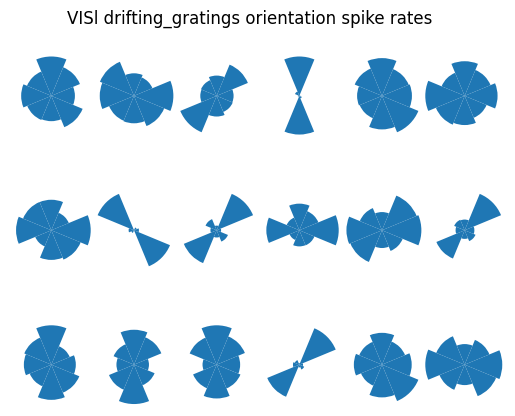
\includegraphics[width=0.6\linewidth]{report_images/drifting_unit_mean_orientation.png}
  \caption{Mean orientation preference of drifting units}
  \label{fig:drifting_unit_mean_orientation}
\end{figure}

One interesting phenomenon is the existence of units which show a response to orientations which are 180° apart.  These units are likely those which respond solely to the orientation and not the drifting.

For this, we define the Direction Sensitivity Index (DSI), which is the same as the OSI, but where \(\bar\theta\) is opposite to \(\theta^*\) as opposed to orthogonal.  Only 8 units among the 81 that were originally chosen exhibited a DSI value greater than 0.5, which supports our hypothesis that these units are more correlated to orientation than to the drifting itself.

\section{Decoding Orientation from Neural Activity}

To assess whether the activity patterns of orientation-selective neurons could reliably predict stimulus orientation, we implemented a machine learning approach using the spike counts of selected neurons as features. The static dataset consisted of spike count responses to static grating stimuli presented at six distinct orientations. Whereas the drifting dataset the same but from 8 distinct orientations as direction is considered. The classification task involved predicting the stimulus orientation from the corresponding neural activity patterns.

\subsection{Data Preparation and Model Training}
We constructed a feature matrix with stimulus presentations as rows and the spike counts of a selected neurons as columns with the orientation values being the target variable. Prior to model training the dataset was stratified and split into training (70\%) and testing (30\%) sets to ensure proportional representation of orientation classes. We ended up with 20 presentations per orientation for static dataset whereas only 5 presentations per orientation for drifting dataset, a limitation to be considered. Features were standardized using z score normalization to account for differences in baseline firing rates. We then considered Random Forest Models, SVM with linear kernel and Logistic Regression.

\subsection{Classification performance}

For static, all models performed with accuracy near 0.85 \ref{tab:static_performance}, while drifting performed with near perfect accuracy \ref{tab:drifting_performance}. In both datasets, logistic regression performed best. The difference in performance can be explained by having more orientation-selective features (81 from 43), with these neurons having higher OSI values, though it must be acknowledged that the resolution changes between grating types, possibly affecting decoding. Moreover, our model is limited by having 5 stimulus presentations for drifting and 20 for static.

\subsection{Cross condition analysis between static and drifting stimuli}

At this point we wanted to dig deeper into the difference in OSI between static and drifting gratings by looking at the distribution of the OSI values \ref{fig:tuning_comparison}. 

\[
\begin{array}{|l|c|c|}
\hline
\textbf{Measure} & \textbf{Static Gratings} & \textbf{Drifting Gratings} \\
\hline
\text{Skewness} & 2.258 & 1.937 \\
\text{Kurtosis} & 5.009 & 3.397 \\
\hline
\end{array}
\]

The distribution is highly non-normal: few neurons have a high OSI and are responsible for interpreting orientation.

Drifting activates more neurons with high OSI overall.

Static distribution has higher kurtosis (5.009 $>$ 3.397) indicating a narrower sharper peak and heavier tails than drifting. This suggests fewer relatively higher tuned neurons: the drifting nature of the grating is a kind of noise which triggers a greater response.

Interestingly we see these results in the feature selection of our random forest models for static and drifting. For static fewer units make up a relatively much larger impact on the models decision than for drifting gratings. As for drifting many units have a high OSI value. 

\subsubsection{Distribution and Overlap of Selective Neurons Across Regions}

The distribution of well-tuned neurons across brain regions is very similar, with approximately twice as many well-tuned neurons for drifting compared to static gratings \ref{fig:tuned_regions}. Notably, VISl appears to have greater relative importance for static stimuli, whereas VISrl is more prominent for drifting. Furthermore, of the 43 units identified as significant for static gratings, 29 were also significant for drifting gratings. This substantial overlap indicates that many of the same neurons are involved in processing orientation for both stimulus types, which aligns with expectations.

\section{Limitations and Further Work}

Comparing model performance between static and drifting gratings is limited by the high discrepancy in resolution: static has 30° and while 45° in drifting. This does not limit comparative analysis for OSI as this uses orthogonal values for stimulus count, the same for both. A comparative study with the same resolution could refine our results.

This investigation was limited to a single session, for a mouse. Repeating the study with other sessions would validate results.

We used gratings to infer how orientation is encoded, but it remains to be validated if other oriented stimuli are similarly encoded.

\section{Conclusion}

It is possible to decode gratings orientation from neural response using spike counts. This method is especially effective in drifting gratings, where units have higher OSI values and are selective. However, OSI values for selective neurons in static gratings are much higher, as is apparent from higher kurtosis, and is confirmed by feature importance in the model.

\newpage

\appendix

\section{Appendix}

\begin{table}[H]
\centering
\begin{tabular}{lr}
\toprule
region & count \\
\midrule
grey   & 558 \\
VISal  &  71 \\
VISp   &  63 \\
VISam  &  60 \\
VISrl  &  44 \\
VISl   &  38 \\
VISpm  &  19 \\
CA1    &  16 \\
CA3    &  15 \\
DG     &   7 \\
\bottomrule
\end{tabular}
\caption{Distribution of units across brain regions.}
\label{tab:regions}
\end{table}

\begin{table}[h]
\centering
\begin{tabular}{lr}
\toprule
region & count \\
\midrule
VISal  & 15 \\
VISl   & 10 \\
VISp   &  9 \\
VISam  &  6 \\
VISrl  &  2 \\
grey   &  1 \\
\bottomrule
\end{tabular}
\caption{Distribution of units chosen for static gratings across brain regions}
\label{tab:chosen-regions-static}
\end{table}

\begin{table}[h]
\centering
\begin{tabular}{lr}
\toprule
region & count \\
\midrule
VISal  & 29 \\
VISp   & 19 \\
VISam  & 13 \\
VISl   & 10 \\
VISrl  &  9 \\
VISpm  &  2 \\
grey   &  1 \\
\bottomrule
\end{tabular}
\caption{Distribution of units chosen for drifting gratings across brain regions}
\label{tab:chosen-regions-drifting}
\end{table}

\begin{figure}[ht]
\centering
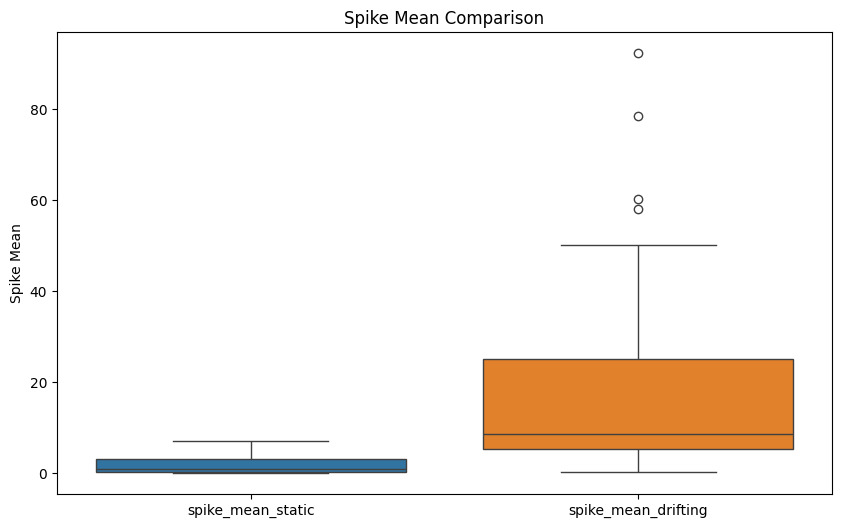
\includegraphics[width=0.85\linewidth]{report_images/spike_mean_comparison.png}
\caption{Spike mean: static and drifting}
\label{fig:spike_mean}
\end{figure}

\begin{figure}[ht]
\centering
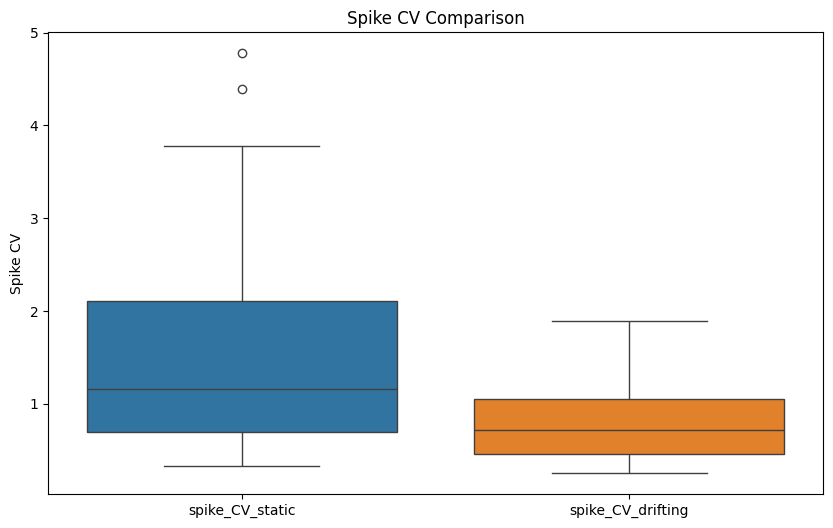
\includegraphics[width=0.85\linewidth]{report_images/spike_CV_comparison.png}
\caption{Spike CV: static and drifting.}
\label{fig:spike_cv}
\end{figure}

\begin{figure}[ht]
\centering
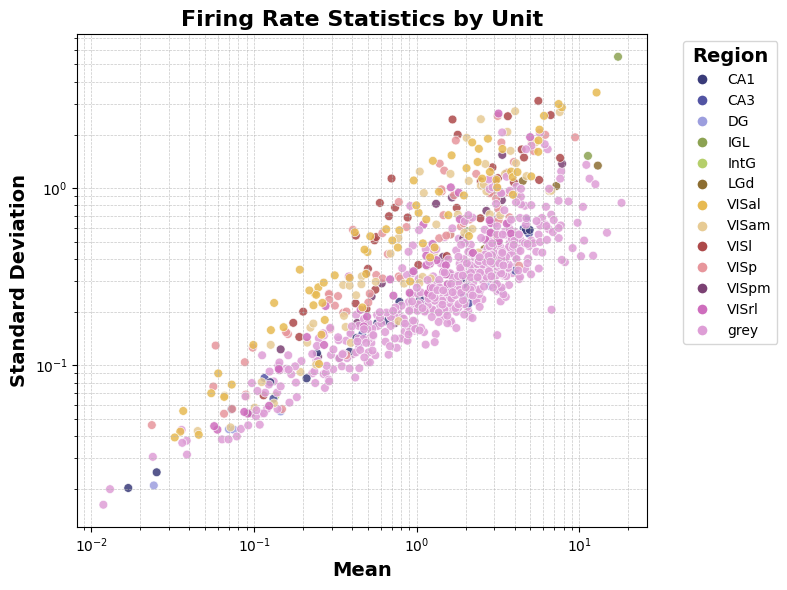
\includegraphics[width=\linewidth]{report_images/unit_firing_rate_statistics.png}
\caption{Firing rate statistics across brain regions.}
\label{fig:firing_rate_stats}
\end{figure}

\begin{figure}[H]
\centering
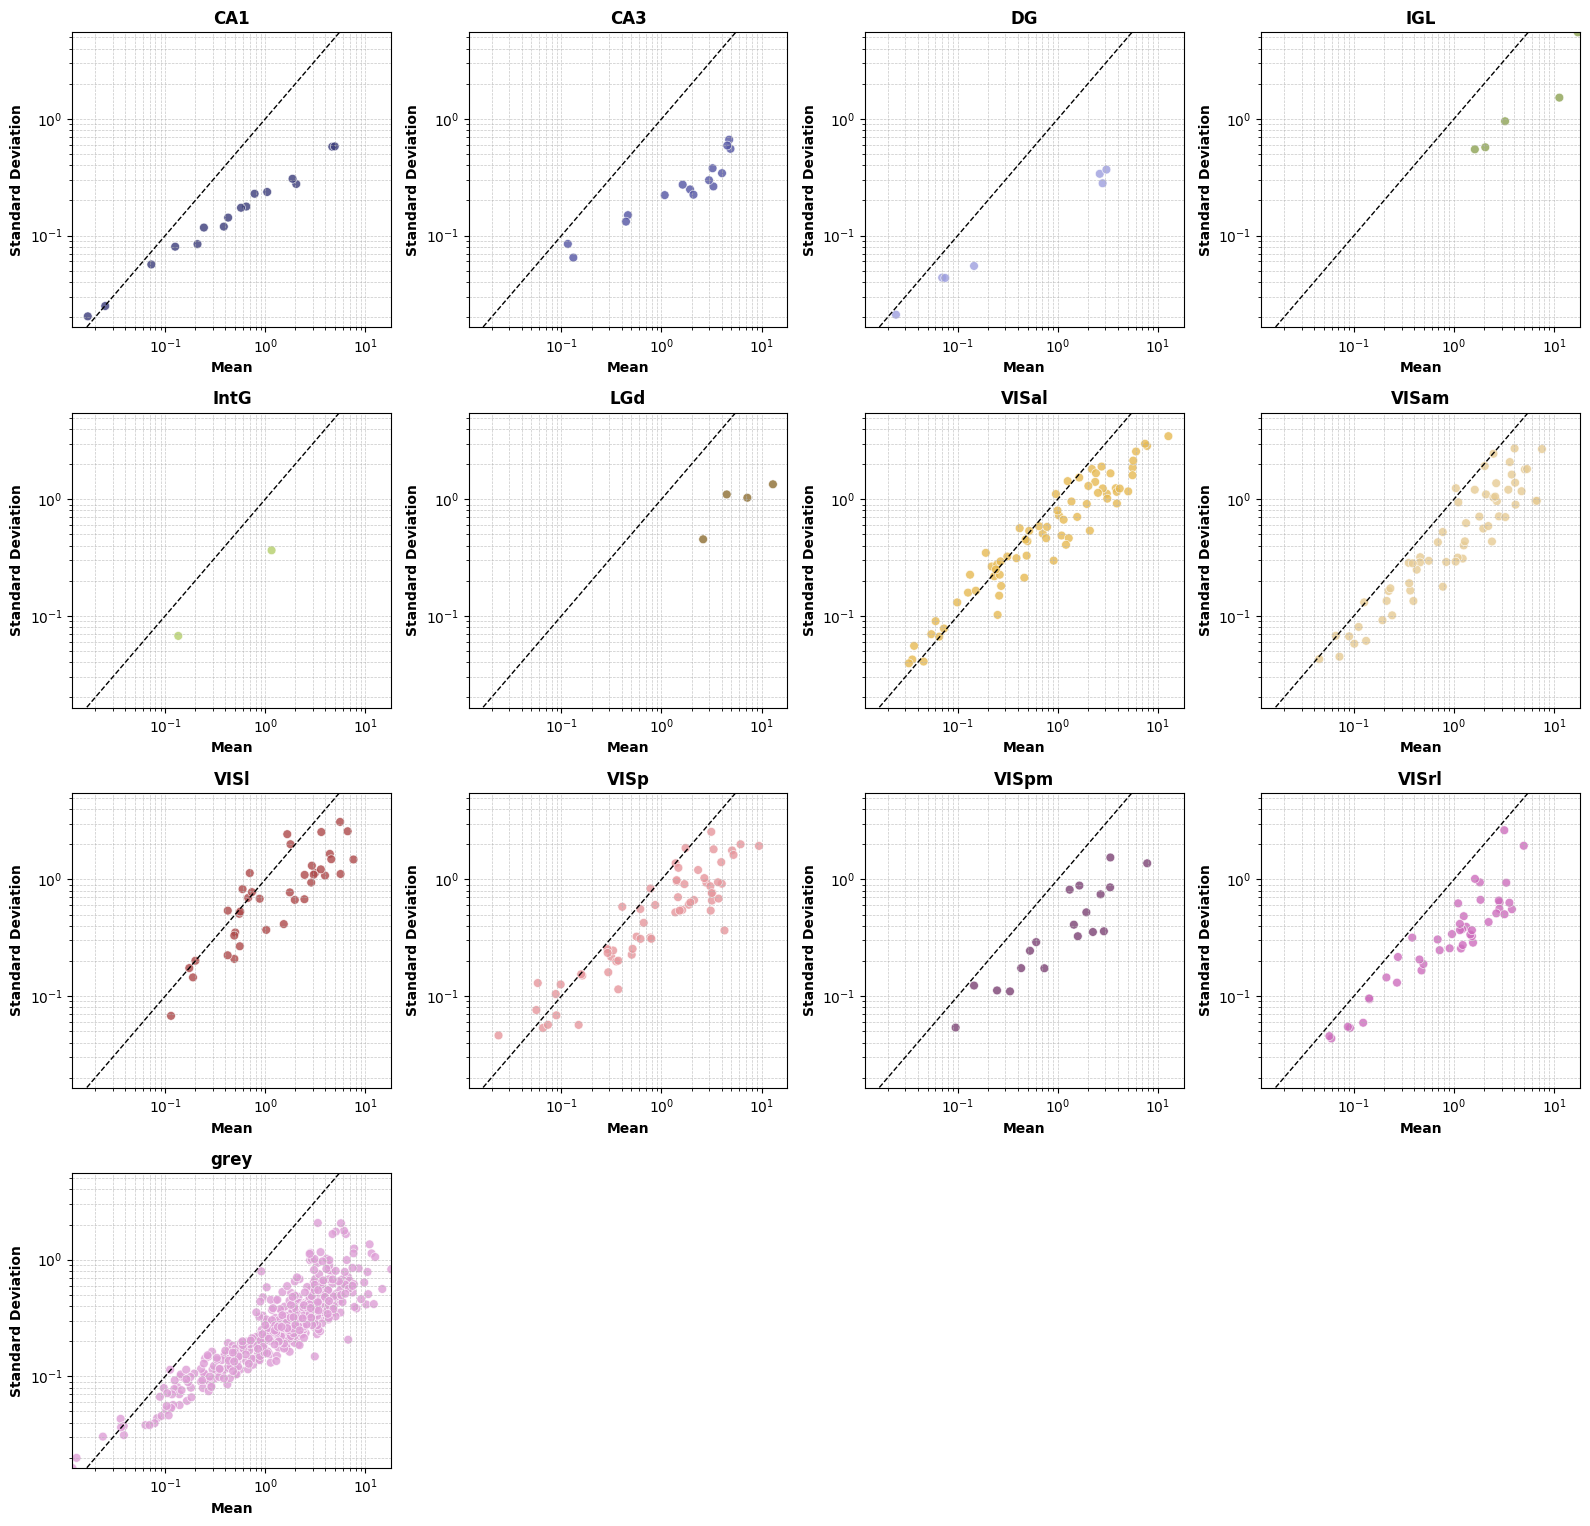
\includegraphics[width=\linewidth]{report_images/unit_firing_rate_statistics_single.png}
\caption{Individual firing rate statistics for each brain region.}
\label{fig:firing_rate_single}
\end{figure}

\begin{figure}[H]
  \centering
  \begin{subfigure}[b]{0.48\linewidth}
    \centering
    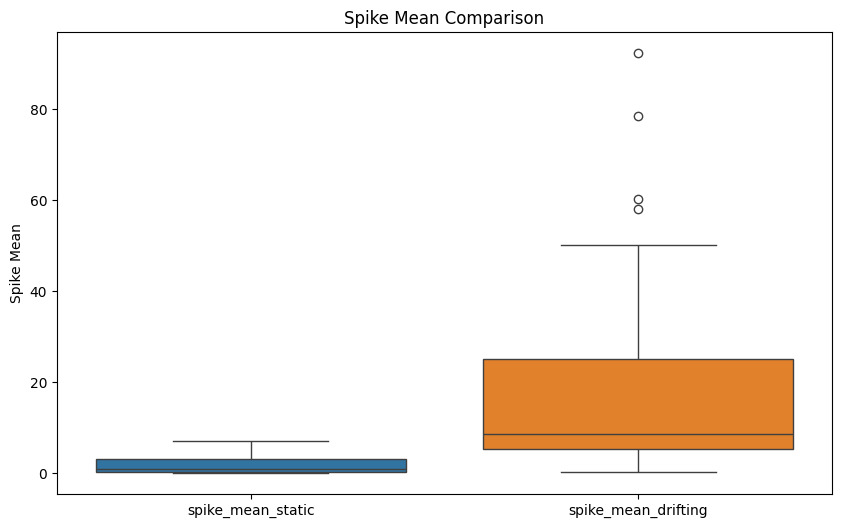
\includegraphics[width=\linewidth]{report_images/spike_mean_comparison.png}
    \caption{Spike mean: static, drifting}
    \label{fig:spike_mean}
  \end{subfigure}
  \hfill
  \begin{subfigure}[b]{0.48\linewidth}
    \centering
    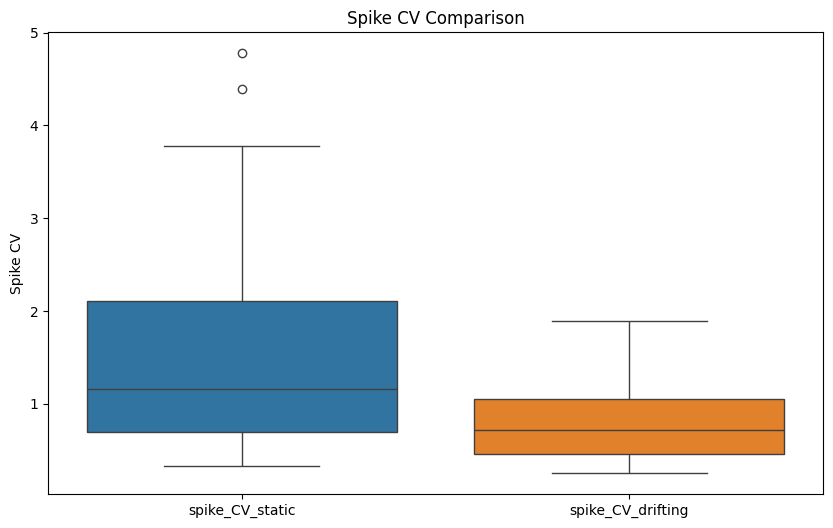
\includegraphics[width=\linewidth]{report_images/spike_CV_comparison.png}
    \caption{Spike CV: static and drifting}
    \label{fig:spike_cv}
  \end{subfigure}
  \caption{Comparison of spike mean and coefficient of variation between static and drifting gratings.}
  \label{fig:spike_stats_comparison}
\end{figure}


\begin{figure}[H]
\centering
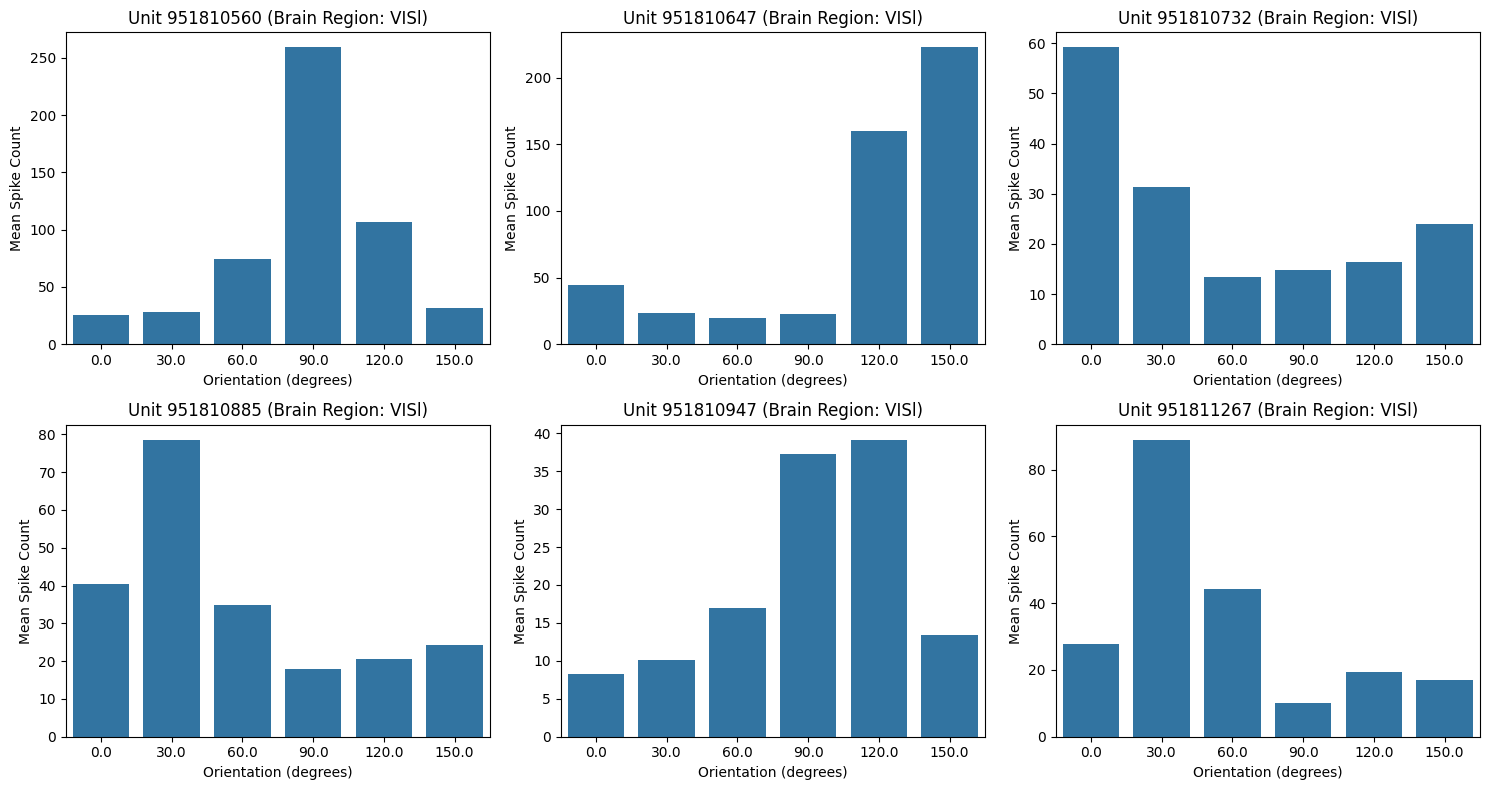
\includegraphics[width=\linewidth]{report_images/static_tuning_curves.png}
\caption{Tuning curves for static gratings.}
\label{fig:static_tuning}
\end{figure}

\begin{figure}[H]
\centering
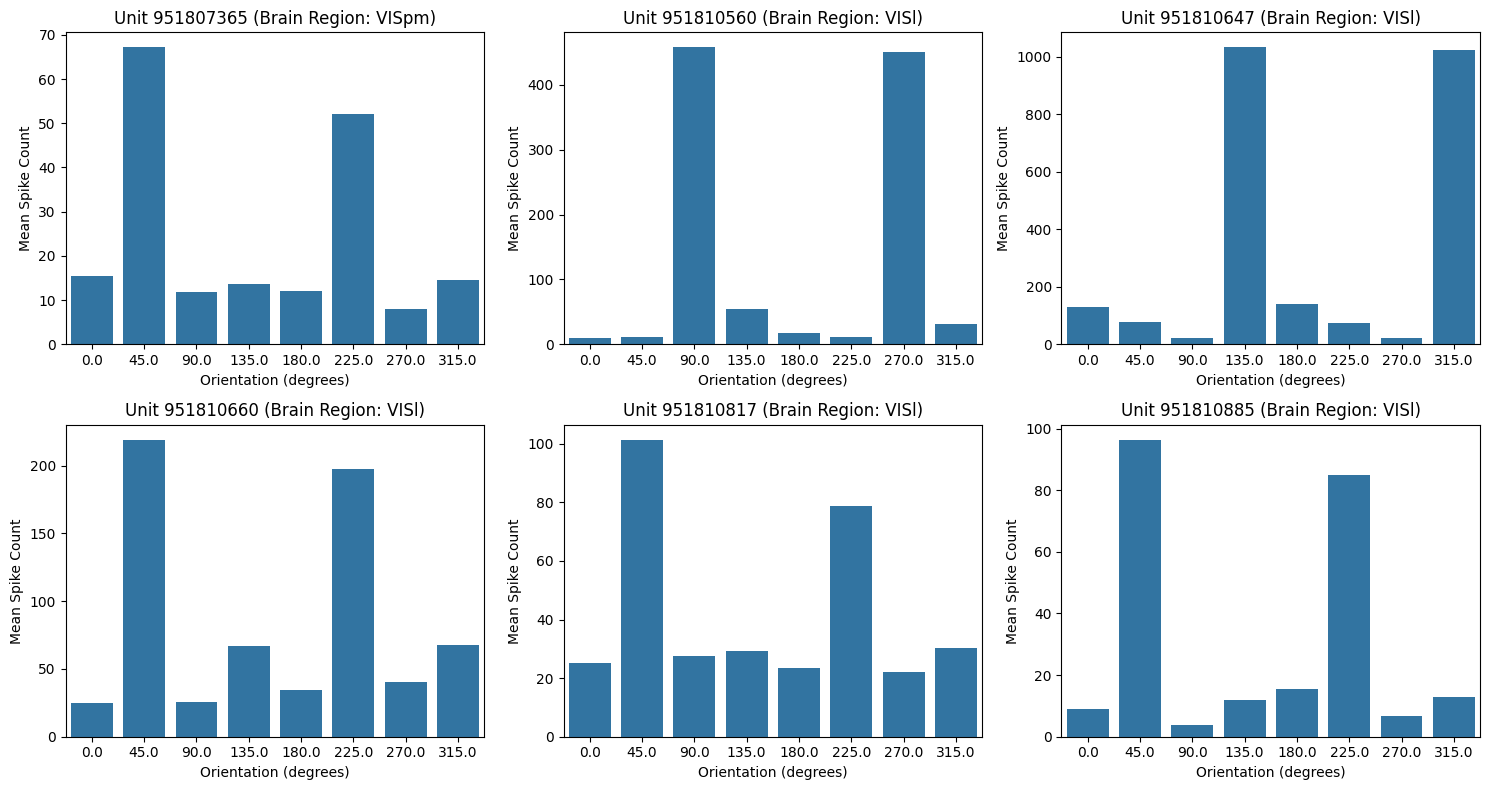
\includegraphics[width=\linewidth]{report_images/Drifting_tuning_curves.png}
\caption{Tuning curves for drifting gratings.}
\label{fig:drifting_tuning}
\end{figure}

\begin{figure}[H]
  \centering
  \begin{subfigure}[b]{0.48\linewidth}
    \centering
    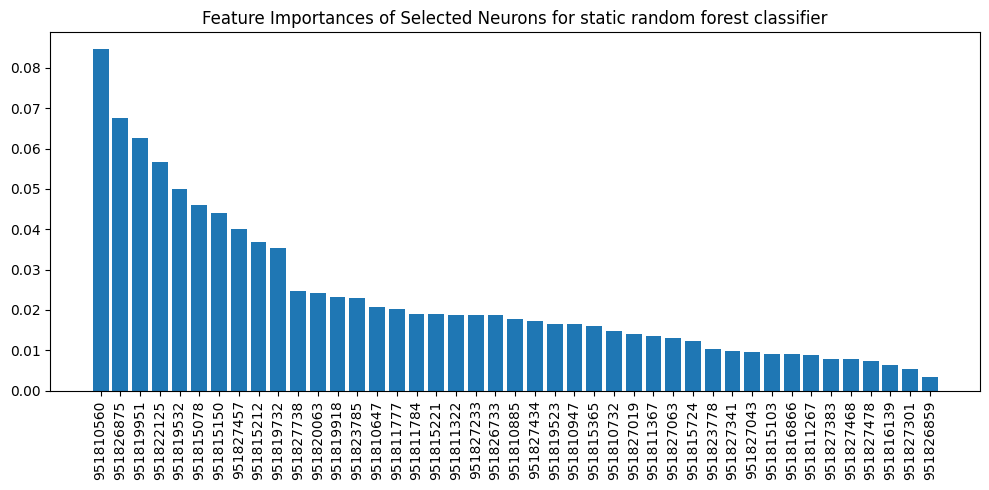
\includegraphics[width=\linewidth]{report_images/static_feature_selection.png}
    \caption{Static gratings}
    \label{fig:static_feature}
  \end{subfigure}
  \hfill
  \begin{subfigure}[b]{0.48\linewidth}
    \centering
    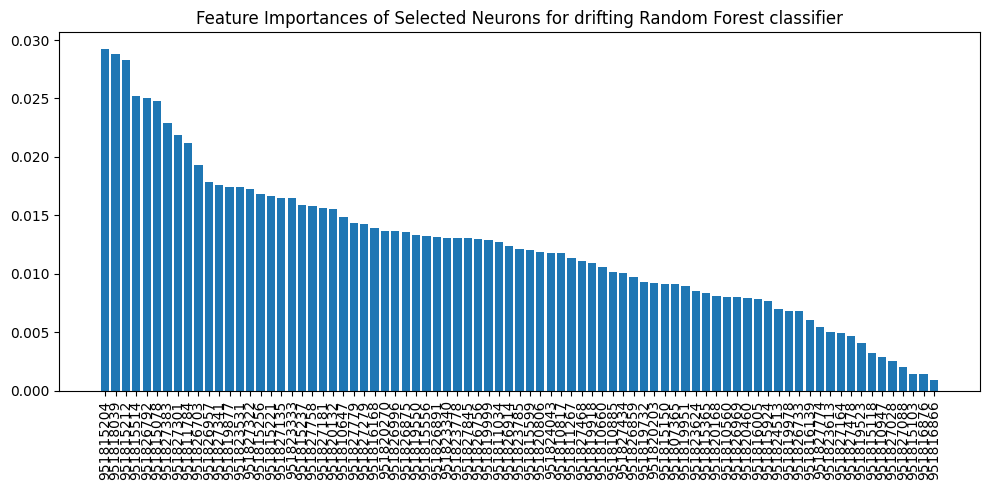
\includegraphics[width=\linewidth]{report_images/drifting_feature_selection.png}
    \caption{Drifting gratings}
    \label{fig:drifting_feature}
  \end{subfigure}
  \caption{Feature selection results for static and drifting gratings.}
  \label{fig:feature_selection_comparison}
\end{figure}


\begin{figure}[H]
  \centering
  \begin{subfigure}[b]{0.48\linewidth}
    \centering
    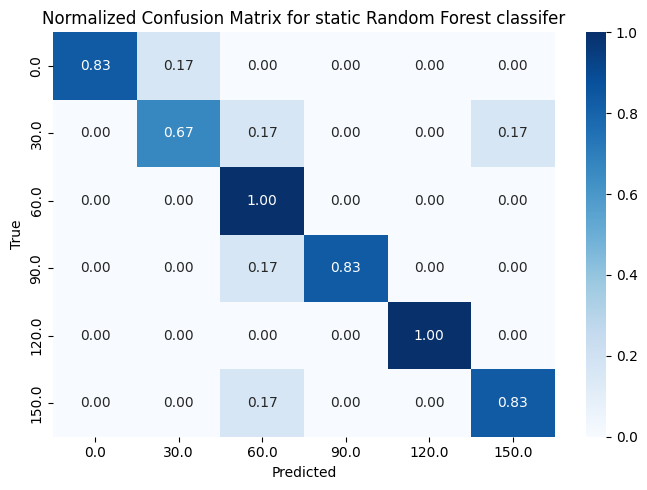
\includegraphics[width=\linewidth]{report_images/static_random_forest_confusion_matrix.png}
    \caption{Static gratings}
    \label{fig:static_rf_cm}
  \end{subfigure}
  \hfill
  \begin{subfigure}[b]{0.48\linewidth}
    \centering
    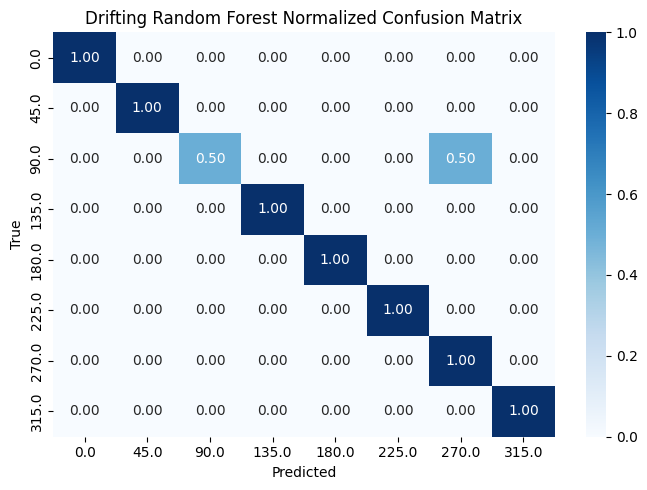
\includegraphics[width=\linewidth]{report_images/drifting_random_forest_confusion_matrix.png}
    \caption{Drifting gratings}
    \label{fig:drifting_rf_cm}
  \end{subfigure}
  \caption{Random Forest confusion matrices for static and drifting gratings.}
  \label{fig:rf_cm_comparison}
\end{figure}  

\begin{figure}[H]
\centering
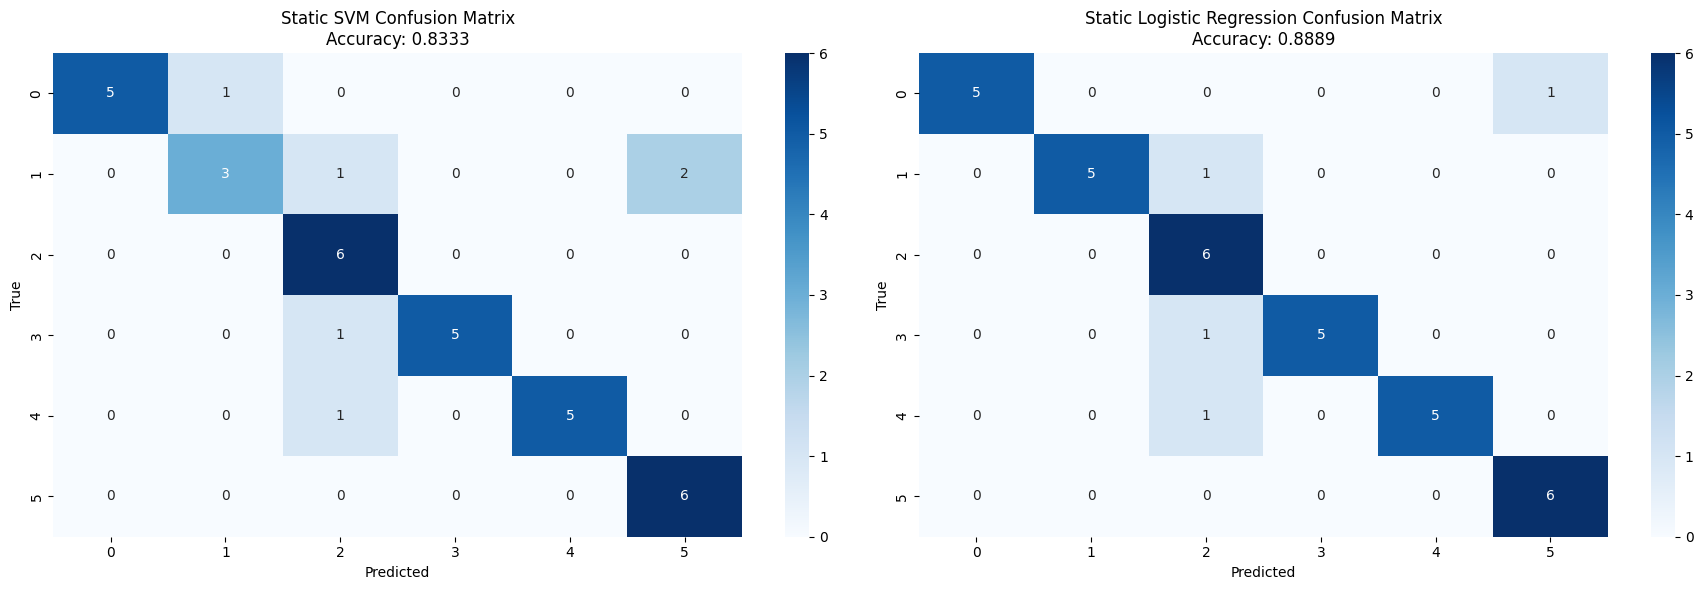
\includegraphics[width=\linewidth]{report_images/static_SVM_LogR_confusion_matrix.png}
\caption{SVM and Logistic Regression confusion matrices for static gratings.}
\label{fig:static_svm_logr_cm}
\end{figure}


\begin{table}[H]
  \centering
  \begin{tabular}{l c}
  \hline
  \textbf{Static} & \textbf{Accuracy} \\
  \hline
  Random Forest        & 0.8611 \\
  SVM                  & 0.8333 \\
  Logistic Regression  & 0.8889 \\
  \hline
  \end{tabular}
  \caption{Classification accuracy for static gratings.}
  \label{tab:static_performance}
  \end{table}
    
  Feature selection for static gratings is visualized in Figure \ref{fig:static_feature} in Appendix A. The confusion matrices for Random Forest, SVM, and Logistic Regression models for static gratings are presented in Figures \ref{fig:static_rf_cm} and \ref{fig:static_svm_logr_cm} in Appendix A.
  
  \begin{table}[H]
  \centering
  \begin{tabular}{l c}
  \hline
  \textbf{Drifting} & \textbf{Accuracy} \\
  \hline
  Random Forest        & 0.9167 \\
  SVM                  & 1.0000 \\
  Logistic Regression  & 1.0000 \\
  \hline
  \end{tabular}
  \caption{Classification accuracy for drifting gratings.}
  \label{tab:drifting_performance}
  \end{table}
  
  Feature selection for drifting gratings is visualized in Figure \ref{fig:drifting_feature} in Appendix A. The confusion matrices for Random Forest, SVM, and Logistic Regression models for drifting gratings are presented in Figures \ref{fig:drifting_rf_cm} and \ref{fig:drifting_svm_logr_cm} in Appendix A.  

\begin{figure}[H]
\centering
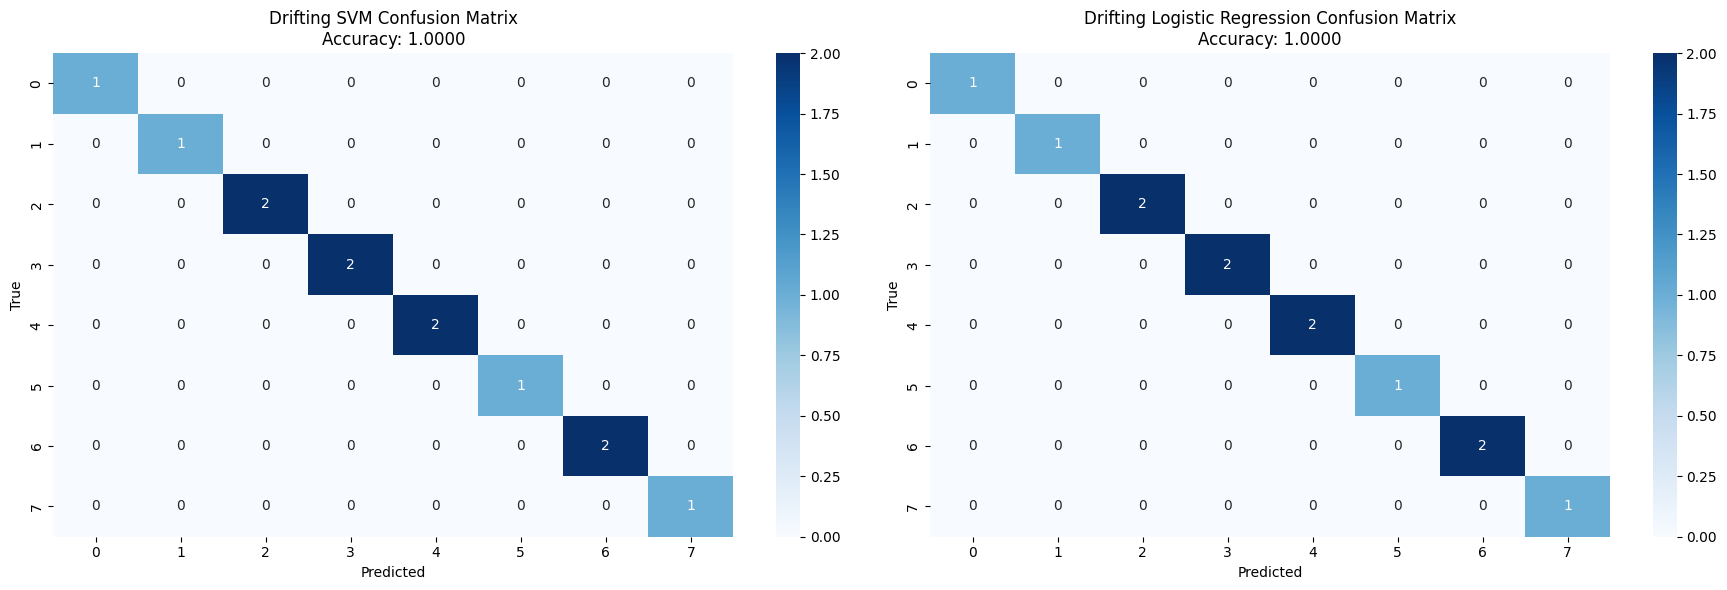
\includegraphics[width=\linewidth]{report_images/drifting_SVM_LogR_confusion_matrix.png}
\caption{SVM and Logistic Regression confusion matrices for drifting gratings.}
\label{fig:drifting_svm_logr_cm}
\end{figure}

\begin{figure}[H]
  \centering
  \begin{subfigure}[b]{0.48\linewidth}
    \centering
    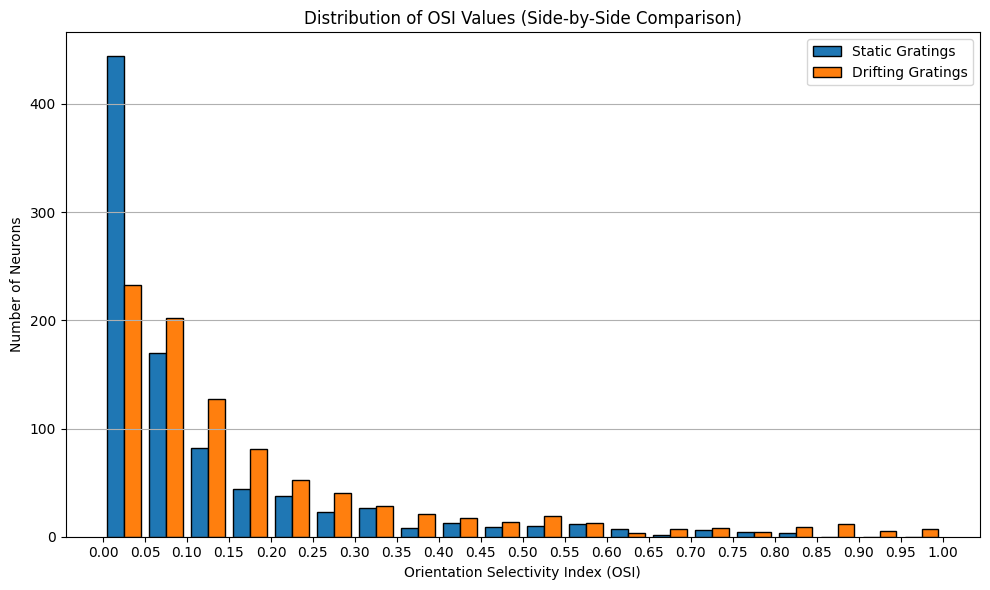
\includegraphics[width=\linewidth]{report_images/tuning_curves_comparison.png}
    \caption{Tuning curves: static vs. drifting.}
    \label{fig:tuning_comparison}
  \end{subfigure}
  \hfill
  \begin{subfigure}[b]{0.48\linewidth}
    \centering
    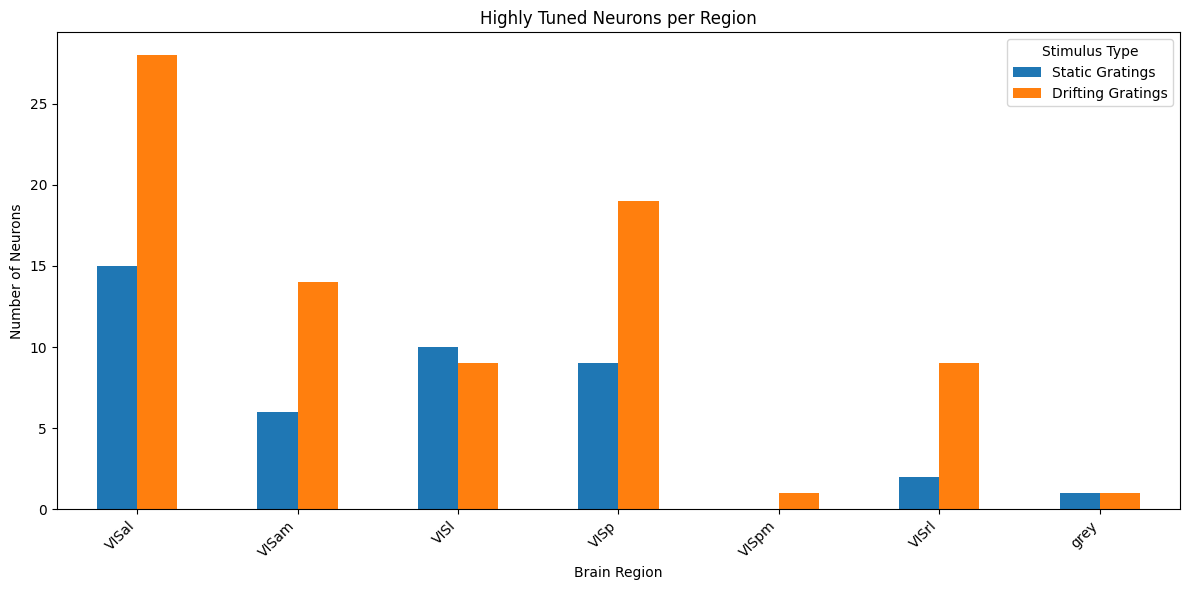
\includegraphics[width=\linewidth]{report_images/tuned_neurons_region.png}
    \caption{Orientation-selective neurons by region.}
    \label{fig:tuned_regions}
  \end{subfigure}
  \caption{Comparison of tuning responses and regional distribution of orientation-selective neurons.}
  \label{fig:tuning_summary}
\end{figure}

\end{document}
